% Created by tikzDevice version 0.12.3.1 on 2022-09-02 10:43:30
% !TEX encoding = UTF-8 Unicode
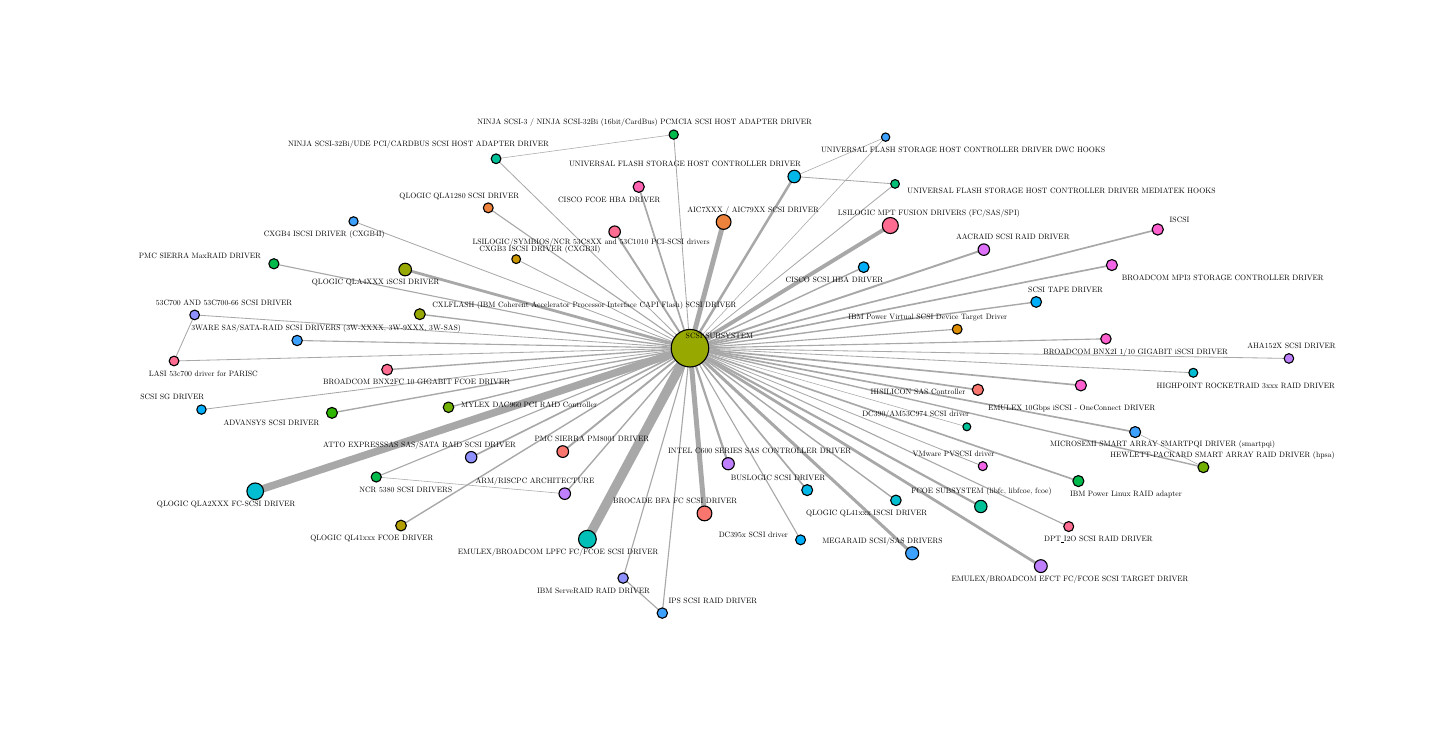
\begin{tikzpicture}[x=1pt,y=1pt]
\definecolor{fillColor}{RGB}{255,255,255}
\path[use as bounding box,fill=fillColor,fill opacity=0.00] (0,0) rectangle (505.89,252.94);
\begin{scope}
\path[clip] (  0.00,  0.00) rectangle (505.89,252.94);
\definecolor{fillColor}{RGB}{255,255,255}

\path[fill=fillColor] (  0.00,  0.00) rectangle (505.89,252.94);
\end{scope}
\begin{scope}
\path[clip] ( 32.75, 32.75) rectangle (475.89,222.94);
\definecolor{drawColor}{gray}{0.66}

\path[draw=drawColor,line width= 0.4pt,line join=round] ( 97.37,139.90) -- (239.32,137.11);

\path[draw=drawColor,line width= 0.3pt,line join=round] ( 60.33,149.14) -- ( 52.89,132.50);

\path[draw=drawColor,line width= 0.3pt,line join=round] ( 60.33,149.14) -- (239.32,137.11);

\path[draw=drawColor,line width= 0.7pt,line join=round] (345.50,172.73) -- (239.32,137.11);

\path[draw=drawColor,line width= 0.5pt,line join=round] (109.95,113.75) -- (239.32,137.11);

\path[draw=drawColor,line width= 0.3pt,line join=round] (455.75,133.41) -- (239.32,137.11);

\path[draw=drawColor,line width= 1.8pt,line join=round] (251.48,182.72) -- (239.32,137.11);

\path[draw=drawColor,line width= 0.2pt,line join=round] (194.07, 84.55) -- (125.95, 90.58);

\path[draw=drawColor,line width= 0.5pt,line join=round] (194.07, 84.55) -- (239.32,137.11);

\path[draw=drawColor,line width= 0.6pt,line join=round] (160.26, 97.72) -- (239.32,137.11);

\path[draw=drawColor,line width= 0.5pt,line join=round] (129.89,129.36) -- (239.32,137.11);

\path[draw=drawColor,line width= 0.4pt,line join=round] (389.63,140.50) -- (239.32,137.11);

\path[draw=drawColor,line width= 0.6pt,line join=round] (391.78,167.16) -- (239.32,137.11);

\path[draw=drawColor,line width= 1.8pt,line join=round] (244.57, 77.41) -- (239.32,137.11);

\path[draw=drawColor,line width= 0.6pt,line join=round] (281.68, 85.83) -- (239.32,137.11);

\path[draw=drawColor,line width= 0.6pt,line join=round] (220.80,195.43) -- (239.32,137.11);

\path[draw=drawColor,line width= 0.5pt,line join=round] (302.09,166.40) -- (239.32,137.11);

\path[draw=drawColor,line width= 0.3pt,line join=round] (176.52,169.29) -- (239.32,137.11);

\path[draw=drawColor,line width= 0.3pt,line join=round] (117.75,182.96) -- (239.32,137.11);

\path[draw=drawColor,line width= 0.5pt,line join=round] (141.69,149.41) -- (239.32,137.11);

\path[draw=drawColor,line width= 0.2pt,line join=round] (339.36,108.71) -- (239.32,137.11);

\path[draw=drawColor,line width= 0.4pt,line join=round] (279.29, 67.86) -- (239.32,137.11);

\path[draw=drawColor,line width= 0.4pt,line join=round] (376.18, 72.67) -- (239.32,137.11);

\path[draw=drawColor,line width= 0.6pt,line join=round] (380.57,123.69) -- (239.32,137.11);

\path[draw=drawColor,line width= 1.0pt,line join=round] (366.10, 58.37) -- (239.32,137.11);

\path[draw=drawColor,line width= 3.4pt,line join=round] (202.26, 68.11) -- (239.32,137.11);

\path[draw=drawColor,line width= 0.8pt,line join=round] (344.42, 79.92) -- (239.32,137.11);

\path[draw=drawColor,line width= 0.2pt,line join=round] (424.84, 94.11) -- (400.19,106.81);

\path[draw=drawColor,line width= 0.5pt,line join=round] (424.84, 94.11) -- (239.32,137.11);

\path[draw=drawColor,line width= 0.3pt,line join=round] (421.19,128.24) -- (239.32,137.11);

\path[draw=drawColor,line width= 0.6pt,line join=round] (343.35,122.08) -- (239.32,137.11);

\path[draw=drawColor,line width= 0.6pt,line join=round] (379.67, 89.10) -- (239.32,137.11);

\path[draw=drawColor,line width= 0.4pt,line join=round] (335.88,143.97) -- (239.32,137.11);

\path[draw=drawColor,line width= 0.4pt,line join=round] (215.15, 54.05) -- (229.32, 41.40);

\path[draw=drawColor,line width= 0.4pt,line join=round] (215.15, 54.05) -- (239.32,137.11);

\path[draw=drawColor,line width= 0.8pt,line join=round] (253.15, 95.37) -- (239.32,137.11);

\path[draw=drawColor,line width= 0.4pt,line join=round] (229.32, 41.40) -- (239.32,137.11);

\path[draw=drawColor,line width= 0.6pt,line join=round] (408.34,180.02) -- (239.32,137.11);

\path[draw=drawColor,line width= 0.3pt,line join=round] ( 52.89,132.50) -- (239.32,137.11);

\path[draw=drawColor,line width= 1.4pt,line join=round] (311.72,181.44) -- (239.32,137.11);

\path[draw=drawColor,line width= 0.7pt,line join=round] (212.10,179.21) -- (239.32,137.11);

\path[draw=drawColor,line width= 1.1pt,line join=round] (319.61, 63.00) -- (239.32,137.11);

\path[draw=drawColor,line width= 0.6pt,line join=round] (400.19,106.81) -- (239.32,137.11);

\path[draw=drawColor,line width= 0.5pt,line join=round] (152.06,115.77) -- (239.32,137.11);

\path[draw=drawColor,line width= 0.4pt,line join=round] (125.95, 90.58) -- (239.32,137.11);

\path[draw=drawColor,line width= 0.2pt,line join=round] (233.44,214.30) -- (169.25,205.56);

\path[draw=drawColor,line width= 0.3pt,line join=round] (233.44,214.30) -- (239.32,137.11);

\path[draw=drawColor,line width= 0.3pt,line join=round] (169.25,205.56) -- (239.32,137.11);

\path[draw=drawColor,line width= 0.4pt,line join=round] ( 88.97,167.62) -- (239.32,137.11);

\path[draw=drawColor,line width= 0.7pt,line join=round] (193.35, 99.76) -- (239.32,137.11);

\path[draw=drawColor,line width= 0.5pt,line join=round] (134.91, 73.02) -- (239.32,137.11);

\path[draw=drawColor,line width= 0.5pt,line join=round] (313.73, 82.14) -- (239.32,137.11);

\path[draw=drawColor,line width= 0.4pt,line join=round] (166.43,187.83) -- (239.32,137.11);

\path[draw=drawColor,line width= 2.7pt,line join=round] ( 82.22, 85.41) -- (239.32,137.11);

\path[draw=drawColor,line width= 1.0pt,line join=round] (136.41,165.54) -- (239.32,137.11);

\path[draw=drawColor,line width= 0.3pt,line join=round] ( 62.79,114.93) -- (239.32,137.11);

\path[draw=drawColor,line width= 0.5pt,line join=round] (239.32,137.11) -- (364.43,153.83);

\path[draw=drawColor,line width= 0.9pt,line join=round] (239.32,137.11) -- (276.99,199.15);

\path[draw=drawColor,line width= 0.2pt,line join=round] (239.32,137.11) -- (310.01,213.38);

\path[draw=drawColor,line width= 0.3pt,line join=round] (239.32,137.11) -- (313.43,196.48);

\path[draw=drawColor,line width= 0.3pt,line join=round] (239.32,137.11) -- (345.12, 94.50);

\path[draw=drawColor,line width= 0.2pt,line join=round] (276.99,199.15) -- (310.01,213.38);

\path[draw=drawColor,line width= 0.3pt,line join=round] (276.99,199.15) -- (313.43,196.48);
\definecolor{drawColor}{RGB}{0,0,0}
\definecolor{fillColor}{RGB}{61,161,255}

\path[draw=drawColor,line width= 0.4pt,line join=round,line cap=round,fill=fillColor] ( 97.37,139.90) circle (  1.88);
\definecolor{fillColor}{RGB}{143,145,255}

\path[draw=drawColor,line width= 0.4pt,line join=round,line cap=round,fill=fillColor] ( 60.33,149.14) circle (  1.75);
\definecolor{fillColor}{RGB}{222,113,249}

\path[draw=drawColor,line width= 0.4pt,line join=round,line cap=round,fill=fillColor] (345.50,172.73) circle (  2.08);
\definecolor{fillColor}{RGB}{47,182,0}

\path[draw=drawColor,line width= 0.4pt,line join=round,line cap=round,fill=fillColor] (109.95,113.75) circle (  1.98);
\definecolor{fillColor}{RGB}{190,128,255}

\path[draw=drawColor,line width= 0.4pt,line join=round,line cap=round,fill=fillColor] (455.75,133.41) circle (  1.73);
\definecolor{fillColor}{RGB}{236,130,60}

\path[draw=drawColor,line width= 0.4pt,line join=round,line cap=round,fill=fillColor] (251.48,182.72) circle (  2.67);
\definecolor{fillColor}{RGB}{190,128,255}

\path[draw=drawColor,line width= 0.4pt,line join=round,line cap=round,fill=fillColor] (194.07, 84.55) circle (  2.08);
\definecolor{fillColor}{RGB}{143,145,255}

\path[draw=drawColor,line width= 0.4pt,line join=round,line cap=round,fill=fillColor] (160.26, 97.72) circle (  2.06);
\definecolor{fillColor}{RGB}{255,108,146}

\path[draw=drawColor,line width= 0.4pt,line join=round,line cap=round,fill=fillColor] (129.89,129.36) circle (  1.96);
\definecolor{fillColor}{RGB}{254,97,207}

\path[draw=drawColor,line width= 0.4pt,line join=round,line cap=round,fill=fillColor] (389.63,140.50) circle (  1.88);
\definecolor{fillColor}{RGB}{242,101,231}

\path[draw=drawColor,line width= 0.4pt,line join=round,line cap=round,fill=fillColor] (391.78,167.16) circle (  2.00);
\definecolor{fillColor}{RGB}{248,118,109}

\path[draw=drawColor,line width= 0.4pt,line join=round,line cap=round,fill=fillColor] (244.57, 77.41) circle (  2.67);
\definecolor{fillColor}{RGB}{0,183,232}

\path[draw=drawColor,line width= 0.4pt,line join=round,line cap=round,fill=fillColor] (281.68, 85.83) circle (  1.99);
\definecolor{fillColor}{RGB}{255,100,179}

\path[draw=drawColor,line width= 0.4pt,line join=round,line cap=round,fill=fillColor] (220.80,195.43) circle (  2.02);
\definecolor{fillColor}{RGB}{0,174,250}

\path[draw=drawColor,line width= 0.4pt,line join=round,line cap=round,fill=fillColor] (302.09,166.40) circle (  1.94);
\definecolor{fillColor}{RGB}{202,151,0}

\path[draw=drawColor,line width= 0.4pt,line join=round,line cap=round,fill=fillColor] (176.52,169.29) circle (  1.59);
\definecolor{fillColor}{RGB}{61,161,255}

\path[draw=drawColor,line width= 0.4pt,line join=round,line cap=round,fill=fillColor] (117.75,182.96) circle (  1.66);
\definecolor{fillColor}{RGB}{151,169,0}

\path[draw=drawColor,line width= 0.4pt,line join=round,line cap=round,fill=fillColor] (141.69,149.41) circle (  1.97);
\definecolor{fillColor}{RGB}{0,192,152}

\path[draw=drawColor,line width= 0.4pt,line join=round,line cap=round,fill=fillColor] (339.36,108.71) circle (  1.43);
\definecolor{fillColor}{RGB}{0,174,250}

\path[draw=drawColor,line width= 0.4pt,line join=round,line cap=round,fill=fillColor] (279.29, 67.86) circle (  1.79);
\definecolor{fillColor}{RGB}{255,108,146}

\path[draw=drawColor,line width= 0.4pt,line join=round,line cap=round,fill=fillColor] (376.18, 72.67) circle (  1.80);
\definecolor{fillColor}{RGB}{254,97,207}

\path[draw=drawColor,line width= 0.4pt,line join=round,line cap=round,fill=fillColor] (380.57,123.69) circle (  2.02);
\definecolor{fillColor}{RGB}{190,128,255}

\path[draw=drawColor,line width= 0.4pt,line join=round,line cap=round,fill=fillColor] (366.10, 58.37) circle (  2.32);
\definecolor{fillColor}{RGB}{0,192,183}

\path[draw=drawColor,line width= 0.4pt,line join=round,line cap=round,fill=fillColor] (202.26, 68.11) circle (  3.21);
\definecolor{fillColor}{RGB}{0,192,152}

\path[draw=drawColor,line width= 0.4pt,line join=round,line cap=round,fill=fillColor] (344.42, 79.92) circle (  2.23);
\definecolor{fillColor}{RGB}{113,176,0}

\path[draw=drawColor,line width= 0.4pt,line join=round,line cap=round,fill=fillColor] (424.84, 94.11) circle (  1.98);
\definecolor{fillColor}{RGB}{0,189,209}

\path[draw=drawColor,line width= 0.4pt,line join=round,line cap=round,fill=fillColor] (421.19,128.24) circle (  1.62);
\definecolor{fillColor}{RGB}{248,118,109}

\path[draw=drawColor,line width= 0.4pt,line join=round,line cap=round,fill=fillColor] (343.35,122.08) circle (  2.03);
\definecolor{fillColor}{RGB}{0,187,75}

\path[draw=drawColor,line width= 0.4pt,line join=round,line cap=round,fill=fillColor] (379.67, 89.10) circle (  2.00);
\definecolor{fillColor}{RGB}{221,141,0}

\path[draw=drawColor,line width= 0.4pt,line join=round,line cap=round,fill=fillColor] (335.88,143.97) circle (  1.77);
\definecolor{fillColor}{RGB}{143,145,255}

\path[draw=drawColor,line width= 0.4pt,line join=round,line cap=round,fill=fillColor] (215.15, 54.05) circle (  1.88);
\definecolor{fillColor}{RGB}{190,128,255}

\path[draw=drawColor,line width= 0.4pt,line join=round,line cap=round,fill=fillColor] (253.15, 95.37) circle (  2.20);
\definecolor{fillColor}{RGB}{61,161,255}

\path[draw=drawColor,line width= 0.4pt,line join=round,line cap=round,fill=fillColor] (229.32, 41.40) circle (  1.88);
\definecolor{fillColor}{RGB}{254,97,207}

\path[draw=drawColor,line width= 0.4pt,line join=round,line cap=round,fill=fillColor] (408.34,180.02) circle (  2.04);
\definecolor{fillColor}{RGB}{255,108,146}

\path[draw=drawColor,line width= 0.4pt,line join=round,line cap=round,fill=fillColor] ( 52.89,132.50) circle (  1.75);

\path[draw=drawColor,line width= 0.4pt,line join=round,line cap=round,fill=fillColor] (311.72,181.44) circle (  2.89);

\path[draw=drawColor,line width= 0.4pt,line join=round,line cap=round,fill=fillColor] (212.10,179.21) circle (  2.08);
\definecolor{fillColor}{RGB}{61,161,255}

\path[draw=drawColor,line width= 0.4pt,line join=round,line cap=round,fill=fillColor] (319.61, 63.00) circle (  2.36);

\path[draw=drawColor,line width= 0.4pt,line join=round,line cap=round,fill=fillColor] (400.19,106.81) circle (  2.00);
\definecolor{fillColor}{RGB}{113,176,0}

\path[draw=drawColor,line width= 0.4pt,line join=round,line cap=round,fill=fillColor] (152.06,115.77) circle (  1.90);
\definecolor{fillColor}{RGB}{0,187,75}

\path[draw=drawColor,line width= 0.4pt,line join=round,line cap=round,fill=fillColor] (125.95, 90.58) circle (  1.83);

\path[draw=drawColor,line width= 0.4pt,line join=round,line cap=round,fill=fillColor] (233.44,214.30) circle (  1.68);
\definecolor{fillColor}{RGB}{0,192,152}

\path[draw=drawColor,line width= 0.4pt,line join=round,line cap=round,fill=fillColor] (169.25,205.56) circle (  1.76);
\definecolor{fillColor}{RGB}{0,187,75}

\path[draw=drawColor,line width= 0.4pt,line join=round,line cap=round,fill=fillColor] ( 88.97,167.62) circle (  1.84);
\definecolor{fillColor}{RGB}{248,118,109}

\path[draw=drawColor,line width= 0.4pt,line join=round,line cap=round,fill=fillColor] (193.35, 99.76) circle (  2.11);
\definecolor{fillColor}{RGB}{179,160,0}

\path[draw=drawColor,line width= 0.4pt,line join=round,line cap=round,fill=fillColor] (134.91, 73.02) circle (  1.94);
\definecolor{fillColor}{RGB}{0,189,209}

\path[draw=drawColor,line width= 0.4pt,line join=round,line cap=round,fill=fillColor] (313.73, 82.14) circle (  1.91);
\definecolor{fillColor}{RGB}{236,130,60}

\path[draw=drawColor,line width= 0.4pt,line join=round,line cap=round,fill=fillColor] (166.43,187.83) circle (  1.79);
\definecolor{fillColor}{RGB}{0,189,209}

\path[draw=drawColor,line width= 0.4pt,line join=round,line cap=round,fill=fillColor] ( 82.22, 85.41) circle (  3.01);
\definecolor{fillColor}{RGB}{151,169,0}

\path[draw=drawColor,line width= 0.4pt,line join=round,line cap=round,fill=fillColor] (136.41,165.54) circle (  2.28);
\definecolor{fillColor}{RGB}{0,174,250}

\path[draw=drawColor,line width= 0.4pt,line join=round,line cap=round,fill=fillColor] ( 62.79,114.93) circle (  1.69);
\definecolor{fillColor}{RGB}{151,169,0}

\path[draw=drawColor,line width= 0.4pt,line join=round,line cap=round,fill=fillColor] (239.32,137.11) circle (  6.78);
\definecolor{fillColor}{RGB}{0,174,250}

\path[draw=drawColor,line width= 0.4pt,line join=round,line cap=round,fill=fillColor] (364.43,153.83) circle (  1.94);
\definecolor{fillColor}{RGB}{0,183,232}

\path[draw=drawColor,line width= 0.4pt,line join=round,line cap=round,fill=fillColor] (276.99,199.15) circle (  2.26);
\definecolor{fillColor}{RGB}{61,161,255}

\path[draw=drawColor,line width= 0.4pt,line join=round,line cap=round,fill=fillColor] (310.01,213.38) circle (  1.51);
\definecolor{fillColor}{RGB}{0,191,118}

\path[draw=drawColor,line width= 0.4pt,line join=round,line cap=round,fill=fillColor] (313.43,196.48) circle (  1.57);
\definecolor{fillColor}{RGB}{242,101,231}

\path[draw=drawColor,line width= 0.4pt,line join=round,line cap=round,fill=fillColor] (345.12, 94.50) circle (  1.63);

\node[text=drawColor,anchor=base,inner sep=0pt, outer sep=0pt, scale=  0.28] at (107.85,143.43) {3WARE SAS/SATA-RAID SCSI DRIVERS (3W-XXXX, 3W-9XXX, 3W-SAS)};

\node[text=drawColor,anchor=base,inner sep=0pt, outer sep=0pt, scale=  0.28] at ( 70.95,152.72) {53C700 AND 53C700-66 SCSI DRIVER};

\node[text=drawColor,anchor=base,inner sep=0pt, outer sep=0pt, scale=  0.28] at (355.96,176.27) {AACRAID SCSI RAID DRIVER};

\node[text=drawColor,anchor=base,inner sep=0pt, outer sep=0pt, scale=  0.28] at ( 88.09,109.28) {ADVANSYS SCSI DRIVER};

\node[text=drawColor,anchor=base,inner sep=0pt, outer sep=0pt, scale=  0.28] at (456.67,136.96) {AHA152X SCSI DRIVER};

\node[text=drawColor,anchor=base,inner sep=0pt, outer sep=0pt, scale=  0.28] at (262.12,186.30) {AIC7XXX / AIC79XX SCSI DRIVER};

\node[text=drawColor,anchor=base,inner sep=0pt, outer sep=0pt, scale=  0.28] at (183.30, 88.15) {ARM/RISCPC ARCHITECTURE};

\node[text=drawColor,anchor=base,inner sep=0pt, outer sep=0pt, scale=  0.28] at (141.56,101.27) {ATTO EXPRESSSAS SAS/SATA RAID SCSI DRIVER};

\node[text=drawColor,anchor=base,inner sep=0pt, outer sep=0pt, scale=  0.28] at (140.50,123.82) {BROADCOM BNX2FC 10 GIGABIT FCOE DRIVER};

\node[text=drawColor,anchor=base,inner sep=0pt, outer sep=0pt, scale=  0.28] at (400.35,134.94) {BROADCOM BNX2I 1/10 GIGABIT iSCSI DRIVER};

\node[text=drawColor,anchor=base,inner sep=0pt, outer sep=0pt, scale=  0.28] at (431.85,161.67) {BROADCOM MPI3 STORAGE CONTROLLER DRIVER};

\node[text=drawColor,anchor=base,inner sep=0pt, outer sep=0pt, scale=  0.28] at (233.96, 81.01) {BROCADE BFA FC SCSI DRIVER};

\node[text=drawColor,anchor=base,inner sep=0pt, outer sep=0pt, scale=  0.28] at (271.16, 89.36) {BUSLOGIC SCSI DRIVER};

\node[text=drawColor,anchor=base,inner sep=0pt, outer sep=0pt, scale=  0.28] at (210.13,189.88) {CISCO FCOE HBA DRIVER};

\node[text=drawColor,anchor=base,inner sep=0pt, outer sep=0pt, scale=  0.28] at (291.50,160.88) {CISCO SCSI HBA DRIVER};

\node[text=drawColor,anchor=base,inner sep=0pt, outer sep=0pt, scale=  0.28] at (185.10,171.99) {CXGB3 ISCSI DRIVER (CXGB3I)};

\node[text=drawColor,anchor=base,inner sep=0pt, outer sep=0pt, scale=  0.28] at (107.19,177.41) {CXGB4 ISCSI DRIVER (CXGB4I)};

\node[text=drawColor,anchor=base,inner sep=0pt, outer sep=0pt, scale=  0.28] at (201.17,151.93) {CXLFLASH (IBM Coherent Accelerator Processor Interface CAPI Flash) SCSI DRIVER};

\node[text=drawColor,anchor=base,inner sep=0pt, outer sep=0pt, scale=  0.28] at (320.90,112.28) {DC390/AM53C974 SCSI driver};

\node[text=drawColor,anchor=base,inner sep=0pt, outer sep=0pt, scale=  0.28] at (262.24, 68.57) {DC395x SCSI driver};

\node[text=drawColor,anchor=base,inner sep=0pt, outer sep=0pt, scale=  0.28] at (386.91, 67.09) {DPT{\_{}}I2O SCSI RAID DRIVER};

\node[text=drawColor,anchor=base,inner sep=0pt, outer sep=0pt, scale=  0.28] at (377.25,114.74) {EMULEX 10Gbps iSCSI - OneConnect DRIVER};

\node[text=drawColor,anchor=base,inner sep=0pt, outer sep=0pt, scale=  0.28] at (376.64, 52.87) {EMULEX/BROADCOM EFCT FC/FCOE SCSI TARGET DRIVER};

\node[text=drawColor,anchor=base,inner sep=0pt, outer sep=0pt, scale=  0.28] at (191.68, 62.57) {EMULEX/BROADCOM LPFC FC/FCOE SCSI DRIVER};

\node[text=drawColor,anchor=base,inner sep=0pt, outer sep=0pt, scale=  0.28] at (344.67, 84.56) {FCOE SUBSYSTEM (libfc, libfcoe, fcoe)};

\node[text=drawColor,anchor=base,inner sep=0pt, outer sep=0pt, scale=  0.28] at (431.73, 97.60) {HEWLETT-PACKARD SMART ARRAY RAID DRIVER (hpsa)};

\node[text=drawColor,anchor=base,inner sep=0pt, outer sep=0pt, scale=  0.28] at (440.18,122.71) {HIGHPOINT ROCKETRAID 3xxx RAID DRIVER};

\node[text=drawColor,anchor=base,inner sep=0pt, outer sep=0pt, scale=  0.28] at (321.71,120.33) {HISILICON SAS Controller};

\node[text=drawColor,anchor=base,inner sep=0pt, outer sep=0pt, scale=  0.28] at (396.86, 83.60) {IBM Power Linux RAID adapter};

\node[text=drawColor,anchor=base,inner sep=0pt, outer sep=0pt, scale=  0.28] at (325.26,147.57) {IBM Power Virtual SCSI Device Target Driver};

\node[text=drawColor,anchor=base,inner sep=0pt, outer sep=0pt, scale=  0.28] at (204.46, 48.51) {IBM ServeRAID RAID DRIVER};

\node[text=drawColor,anchor=base,inner sep=0pt, outer sep=0pt, scale=  0.28] at (264.49, 98.97) {INTEL C600 SERIES SAS CONTROLLER DRIVER};

\node[text=drawColor,anchor=base,inner sep=0pt, outer sep=0pt, scale=  0.28] at (247.58, 44.94) {IPS SCSI RAID DRIVER};

\node[text=drawColor,anchor=base,inner sep=0pt, outer sep=0pt, scale=  0.28] at (416.23,182.42) {ISCSI};

\node[text=drawColor,anchor=base,inner sep=0pt, outer sep=0pt, scale=  0.28] at ( 63.50,126.95) {LASI 53c700 driver for PARISC};

\node[text=drawColor,anchor=base,inner sep=0pt, outer sep=0pt, scale=  0.28] at (325.64,185.02) {LSILOGIC MPT FUSION DRIVERS (FC/SAS/SPI)};

\node[text=drawColor,anchor=base,inner sep=0pt, outer sep=0pt, scale=  0.28] at (203.61,174.52) {LSILOGIC/SYMBIOS/NCR 53C8XX and 53C1010 PCI-SCSI drivers};

\node[text=drawColor,anchor=base,inner sep=0pt, outer sep=0pt, scale=  0.28] at (308.89, 66.61) {MEGARAID SCSI/SAS DRIVERS};

\node[text=drawColor,anchor=base,inner sep=0pt, outer sep=0pt, scale=  0.28] at (410.12,101.57) {MICROSEMI SMART ARRAY SMARTPQI DRIVER (smartpqi)};

\node[text=drawColor,anchor=base,inner sep=0pt, outer sep=0pt, scale=  0.28] at (181.20,115.81) {MYLEX DAC960 PCI RAID Controller};

\node[text=drawColor,anchor=base,inner sep=0pt, outer sep=0pt, scale=  0.28] at (136.62, 85.04) {NCR 5380 SCSI DRIVERS};

\node[text=drawColor,anchor=base,inner sep=0pt, outer sep=0pt, scale=  0.28] at (222.93,217.84) {NINJA SCSI-3 / NINJA SCSI-32Bi (16bit/CardBus) PCMCIA SCSI HOST ADAPTER DRIVER};

\node[text=drawColor,anchor=base,inner sep=0pt, outer sep=0pt, scale=  0.28] at (141.23,209.84) {NINJA SCSI-32Bi/UDE PCI/CARDBUS SCSI HOST ADAPTER DRIVER};

\node[text=drawColor,anchor=base,inner sep=0pt, outer sep=0pt, scale=  0.28] at ( 62.23,169.42) {PMC SIERRA MaxRAID DRIVER};

\node[text=drawColor,anchor=base,inner sep=0pt, outer sep=0pt, scale=  0.28] at (203.88,103.40) {PMC SIERRA PM8001 DRIVER};

\node[text=drawColor,anchor=base,inner sep=0pt, outer sep=0pt, scale=  0.28] at (124.36, 67.50) {QLOGIC QL41xxx FCOE DRIVER};

\node[text=drawColor,anchor=base,inner sep=0pt, outer sep=0pt, scale=  0.28] at (303.13, 76.58) {QLOGIC QL41xxx ISCSI DRIVER};

\node[text=drawColor,anchor=base,inner sep=0pt, outer sep=0pt, scale=  0.28] at (155.95,191.37) {QLOGIC QLA1280 SCSI DRIVER};

\node[text=drawColor,anchor=base,inner sep=0pt, outer sep=0pt, scale=  0.28] at ( 71.72, 79.92) {QLOGIC QLA2XXX FC-SCSI DRIVER};

\node[text=drawColor,anchor=base,inner sep=0pt, outer sep=0pt, scale=  0.28] at (125.75,159.98) {QLOGIC QLA4XXX iSCSI DRIVER};

\node[text=drawColor,anchor=base,inner sep=0pt, outer sep=0pt, scale=  0.28] at ( 52.23,118.50) {SCSI SG DRIVER};

\node[text=drawColor,anchor=base,inner sep=0pt, outer sep=0pt, scale=  0.28] at (250.00,140.70) {SCSI SUBSYSTEM};

\node[text=drawColor,anchor=base,inner sep=0pt, outer sep=0pt, scale=  0.28] at (375.04,157.42) {SCSI TAPE DRIVER};

\node[text=drawColor,anchor=base,inner sep=0pt, outer sep=0pt, scale=  0.28] at (237.52,202.71) {UNIVERSAL FLASH STORAGE HOST CONTROLLER DRIVER};

\node[text=drawColor,anchor=base,inner sep=0pt, outer sep=0pt, scale=  0.28] at (338.04,207.88) {UNIVERSAL FLASH STORAGE HOST CONTROLLER DRIVER DWC HOOKS};

\node[text=drawColor,anchor=base,inner sep=0pt, outer sep=0pt, scale=  0.28] at (373.59,193.03) {UNIVERSAL FLASH STORAGE HOST CONTROLLER DRIVER MEDIATEK HOOKS};

\node[text=drawColor,anchor=base,inner sep=0pt, outer sep=0pt, scale=  0.28] at (334.59, 98.03) {VMware PVSCSI driver};
\end{scope}
\end{tikzpicture}
